\documentclass{article}

\usepackage[english]{babel}
\usepackage[letterpaper,top=2cm,bottom=2cm,left=3cm,right=3cm,marginparwidth=1.75cm]{geometry}

\usepackage{amsmath}
\usepackage{graphicx}
\usepackage{float}
\usepackage[colorlinks=true, allcolors=blue]{hyperref}

\title{Calibration Tool - Setup Manual}
\author{Lovicourt Léo}

\begin{document}
\maketitle

\section{Windows setup}

In a first time, you will have to download the C/C\texttt{++} compiler \href{https://www.mingw-w64.org/downloads/}{MinGW} (\textit{MingW-W64-builds} package). During installation, choose the \textit{posix} threads and the \textit{seh} exception. Once the installation is done, you have to add a variable to the environment variable \textit{"Path"}.\bigskip

Then, there are 2 ways for setting up every library used for the program.
For both, extract the archive in a folder of your choice.

\subsection{Using the files provided in the folder}

There is nothing to install : all the necessary dynamic libraries (\textit{DLL} files) and header files (\textit{h} and \textit{hpp} files) are already provided in the folders \textit{libs} and \textit{include}. However, if you have to add new functionalities, you may have to install the libraries figuring in the next section.

\subsection{Installing the required libraries}

You will have to install 2 libraries : \href{https://opencv.org/releases/}{OpenCV} (4.X) and \href{https://www.wxwidgets.org/downloads/}{wxWidgets} (3.X).\bigskip

For OpenCV, you should not download the Windows executable file as it does not contain the \textit{contrib} modules. Instead, download the source files and build it manually (with \textit{CMake} for example). While building the binaries, don't forget to add the \textit{contrib} modules by adding a path to the \textit{opencv\_contrib/modules} folder. If you use the CMake GUI, you will be able to provide this path directly with the option \textit{OPENCV\_EXTRA\_MODULES\_PATH}.

\begin{figure}[H]
\centering
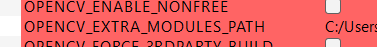
\includegraphics[width=0.5\textwidth]{cmake_gui_contrib.png}
\caption{\label{fig:cmake_gui_contrib}Adding extra modules in CMake GUI.}
\end{figure}

If you build the binaries from command-line, you will have to add this path manually with the option :

\begin{figure}[H]
\centering
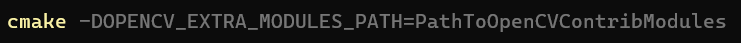
\includegraphics[width=0.5\textwidth]{cmake_terminal_contrib.png}
\caption{\label{fig:cmake_terminal_contrib}Adding extra modules in command-line.}
\end{figure}

For wxWidgets, it is also recommanded (but not necessary) to build the binaries manually by downloading the Windows ZIP from the downloads page. You can use CMake again to build the binaries, and then proceed to the next step.\bigskip


Finally, you will have to define multiple environment variables.\bigskip

\textit{Note : If you do not create these variables, the makefile will use the \texttt{include} and \texttt{libs} provided in the folder.}

For OpenCV, you will have to define the variable \textit{OPENCVB\_DIR}, and add the path to the \texttt{include} folder of OpenCV to this variable. This is the variable used for compiling the source files using OpenCV. You will also have to create the variable \textit{OPENCVL\_DIR} and add the path to the \texttt{bin} folder : we use this variable for the linking process.\bigskip

For wxWidgets, you will again have to create at least 2 environment variables. Create the \textit{WXB\_DIR} and add the path to the \texttt{include} folder of wxWidgets. You may also have to add the \textit{WXSETUP\_DIR} variable and give it the path to the \texttt{setup.h} file, depending on how you installed the library. Most of the time, it will be located in the \texttt{lib} folder of wxWidgets or one of its subfolders. You will finally have to create the variable \textit{WXL\_DIR} and add the path to the \texttt{lib} folder of wxWidgets to the variable.\bigskip

\section{Linux distributions setup}

On a Linux distribution, you will have to install the wxWidgets and OpenCV libraries.\bigskip

You can follow this \href{https://docs.opencv.org/3.4/d7/d9f/tutorial_linux_install.html}{tutorial} for setting up OpenCV. It is important in this tutorial to not forget to add the option \textit{OPENCV\_EXTRA\_MODULES\_PATH} with the correct path while configuring with CMake.


Note that if you install OpenCV without using \texttt{pkg-config} as shown in the tutorial, you may have to edit the makefile to compile the source files.\bigskip


For wxWidgets, you can follow this \href{https://www.binarytides.com/install-wxwidgets-ubuntu/}{tutorial}. If nothing went wrong, you should now be able to compile the source files and create the executable using \texttt{make} in command-line.

\section{Program structure}

\subsection{Folders organisation}

The folder contains several subfolders, each containing specific files.

\begin{itemize}
    \item \textbf{bin} : contains the binary files : the executable setup for Windows OS and the Debian package for Linux distributions.
    \item \textbf{docs} : contains the user manual and the technical manual -- this file.
    \item \textbf{headers} : contains all the headers files (\textit{.hpp} files).
    \item \textbf{include} : contains the content of the \texttt{include} folders of OpenCV and wxWidgets.
    \item \textbf{installer} : contains the NSI script used for building the Windows installer.
    \item \textbf{libs} : contains the libraries required for linking and running the program on Windows OS (\textit{.dll} files).
    \item \textbf{obj} : contains the object files (\textit{.o} files) created during compilation.
    \item \textbf{resource} : contains the software icon and the resource file (\textit{.rc} file).
    \item \textbf{src} : contains the source files (\textit{.cpp} files). 
\end{itemize}

\subsection{Source/header files organisation}

Every source file (\textit{.cpp} file) has its corresponding header file (\textit{.hpp} file). This way, we have a lower compilation time, and we can re-use elements defined in a header file in any source file. This is also a way to prevent cross-referencing while using functions included from these header files.\bigskip


One of the source files (\texttt{App.cpp}) does not have a header file, as its code is very short and is not subject to any big changes.
Also, one of the header files (\texttt{structs.hpp}) does not match any source file : this header contains only the structures declarations, and some macroconstants.\bigskip


In each header file matching a source file, there is a short description above the code explaining what this file contains. Finally, each source file matching a header file implements functions declared in this header.

\section{Compilation and Makefile options}

\subsection{Windows OS}

Type \textbf{mingw32-make} in a terminal opened in the project folder to compile the source files. If you want to remove the executable file and the object files, you can type \textbf{mingw32-make clean} but if you only want to delete the object files, type \textbf{mingw32-make clean\_objs}.

\subsection{Linux distributions}

Type \textbf{make} in a terminal opened in the project folder to compile the source files. If you want to remove the executable file and the object files, you can type \textbf{make clean} but if you only want to delete the object files, type \textbf{make clean\_objs}.


\end{document}